%%%%%%%%%%%%%%%%%%%%%%%%%%%%%%%%%%%%%%%%%
% Beamer Presentation
% LaTeX Template
% Version 1.0 (10/11/12)
%
% This template has been downloaded from:
% http://www.LaTeXTemplates.com
%
% License:
% CC BY-NC-SA 3.0 (http://creativecommons.org/licenses/by-nc-sa/3.0/)
%
%%%%%%%%%%%%%%%%%%%%%%%%%%%%%%%%%%%%%%%%%

%----------------------------------------------------------------------------------------
%	PACKAGES AND THEMES
%----------------------------------------------------------------------------------------
\documentclass[usenames,dvipsnames]{beamer}
%\documentclass{beamer}

\mode<presentation> {
\setbeamercovered{dynamic}%highlits the next pause item/paragraph etc
% The Beamer class comes with a number of default slide themes
% which change the colors and layouts of slides. Below this is a list
% of all the themes, uncomment each in turn to see what they look like.
\definecolor{olive}{rgb}{0.0,0.6,0.0}%able to use dark green color
%\usetheme{default}
%\usetheme{AnnArbor}
%\usetheme{Antibes}
%\usetheme{Bergen}
%\usetheme{Berkeley}
%\usetheme{Berlin}%Very good style
%\usetheme{Boadilla}
%\usetheme{CambridgeUS}
%\usetheme{Copenhagen}
%\usetheme{Darmstadt}
\usetheme{Dresden}
%\usetheme{Frankfurt}
%\usetheme{Goettingen}
%\usetheme{Hannover}
%\usetheme{Ilmenau}
%\usetheme{JuanLesPins}
%\usetheme{Luebeck}
%\usetheme{Madrid}%This was the first form
%\usetheme{Malmoe}
%\usetheme{Marburg}
%\usetheme{Montpellier}
%\usetheme{PaloAlto}
%\usetheme{Pittsburgh}
%\usetheme{Rochester}
%\usetheme{Singapore}
%\usetheme{Szeged}
%\usetheme{Warsaw}

% As well as themes, the Beamer class has a number of color themes
% for any slide theme. Uncomment each of these in turn to see how it
% changes the colors of your current slide theme.

%\usecolortheme{albatross}
%\usecolortheme{beaver}
%\usecolortheme{beetle}
%\usecolortheme{crane}
%\usecolortheme{dolphin}
%\usecolortheme{dove}
%\usecolortheme{fly}
%\usecolortheme{lily}
%\usecolortheme{orchid}
%\usecolortheme{rose}
%\usecolortheme{seagull}
%\usecolortheme{seahorse}
%\usecolortheme{whale}
%\usecolortheme{wolverine}

%\setbeamertemplate{footline} % To remove the footer line in all slides uncomment this line
\setbeamertemplate{footline}[frame number] % To replace the footer line in all slides with a simple slide count uncomment this line
%\setbeamerfont{frametitle}{size=\tiny} %reduces frame size for warsaw, for berlin it only reduces font size
%\setbeamertemplate{navigation symbols}{} % To remove the navigation symbols from the bottom of all slides uncomment this line
}

\usepackage{graphicx} % Allows including images
\usepackage{booktabs} % Allows the use of \toprule, \midrule and \bottomrule in tables
\usepackage{appendixnumberbeamer} % Allows the backupslides not to be counted
\usepackage{xcolor}%to define textcolor
\usepackage{listings}%for code display
%----------------------------------------------------------------------------------------
%	TITLE PAGE
%----------------------------------------------------------------------------------------

\title[Data Science]{Crime in Montgomery county} % The short title appears at the bottom of every slide, the full title is only on the title page

\author{Dawit H. Hailu} % Your name

\institute[Montgomery  College ] % Your institution as it will appear on the bottom of every slide, may be shorthand to save space
{

    \graphicspath{{Figures//}}
     \includegraphics[width=0.6 in]{MClogo.eps}\\ 
    
\medskip
\textit{dhailu@montgomerycollege.edu} \\% Your email address

}
\date{Immersive Data Analytics Bootcamp\ April, 2020} % Date, can be changed to a custom date

\begin{document}

\begin{frame}[noframenumbering]
\titlepage % Print the title page as the first slide
\thispagestyle{empty}
\end{frame}
%----------------------------------------------------------------------------------------
%----------------------------------------------------------------------------------------
\begin{frame}[noframenumbering]
\frametitle{Outline} % Table of contents slide, comment this block out to remove it
\small
\tableofcontents %[pausesections]% Throughout your presentation, if you choose to use \section{} and \subsection{} commands, these will automatically be printed on this slide as an overview of your presentation, [pausesections] pause sections in TOC
\thispagestyle{empty}
\end{frame}
%----------------------------------------------------------------------------------------
\section{Introduction}
\subsection{Project aim}
%----------------------------------------------------------------------------------------
\begin{frame}
\frametitle{}
\begin{block}{The problem}
\begin{itemize}
 \item I want to have a look at crimes in Montgomery county 
 \item This information is believed to help  fight crime and can be used as input for site selection (residence, bussiness)
 \end{itemize}
\end{block}
\begin{block}{aim}
Let us achieve our aim by making use of our newly acquired data science tools
\end{block}
\end{frame}
%------------------------------------------------
%------------------------------------------------
\section{Data Acquisition}
\subsection{Collecting Data}
%------------------------------------------------
%------------------------------------------------------
\begin{frame}
\frametitle{Data Collection}
\begin{itemize} 
\item Data is collected from Montgomery County open data website:\footnote{(https://data.montgomerycountymd.gov/)}
\item Then wrangle, clean it, and read it into a \textcolor{red}{\emph{pandas}} dataframe before making use of it 
\item Consult for the website for data description (meaning of column names)
\end{itemize}
\end{frame}
%------------------------------------------------
%------------------------------------------------

%------------------------------------------------
\begin{frame}
\frametitle{Snippet of the dataset}
%------------------------------------------------
\begin{itemize}
\item Dataframe has \textcolor{red}{202094} rows and \textcolor{red}{30} columns
\item redundant information about location is observed, so I will drop that
\item I will focus on columns with information regarding \textcolor{red}{ crime time} rows and \textcolor{red}{crime district} 
\item Information about time is encoded as \textcolor{red}{ dispatch time} , \textcolor{red}{ start time} and \textcolor{red}{end times} 
\item There are missing entries on the dataset
\end{itemize}

\end{frame}
%------------------------------------------------
\section{Analyzing Crime Patterns}
\subsection{When do crimes happen?}
%------------------------------------------------
%------------------------------------------------------
%\section{Conclusion}
%------------------------------------------------
\begin{frame}
\frametitle{Crime day}
\vspace{-0.5cm}
Based on  \textcolor{blue}{Dispatch},  \textcolor{red}{End}, and  \textcolor{OliveGreen}{Start} time data  \\ 
%Plot of Crime frequency vs days 
\graphicspath{{Figures//}}
%\vspace{-0.5cm}
\begin{figure}[htbp]
%\begin{minipage}[b]{0.5\linewidth}
\centering
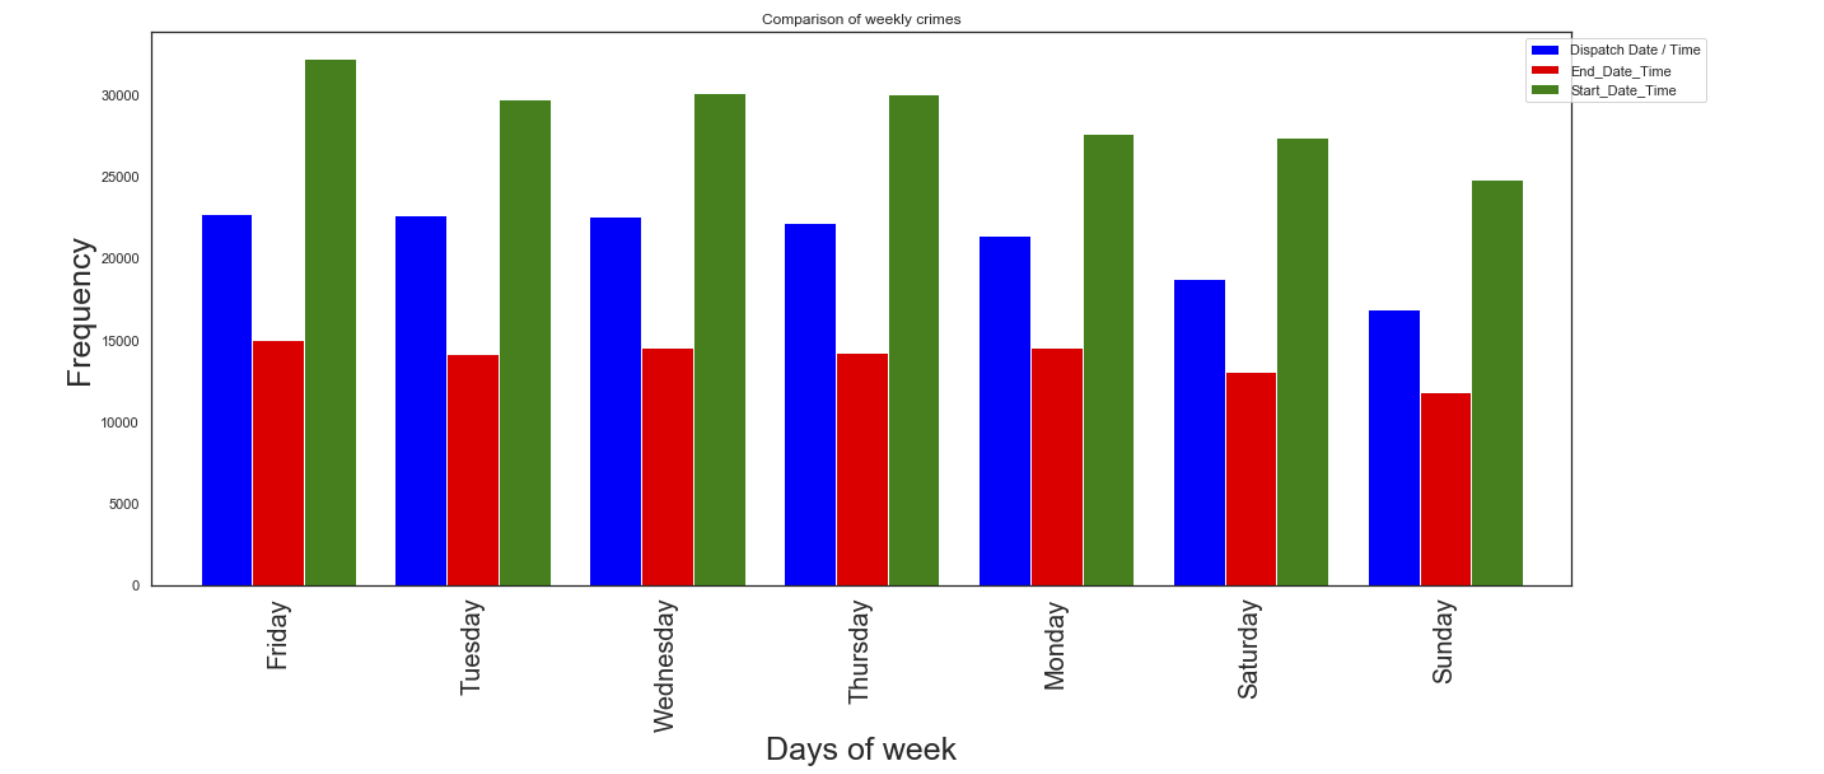
\includegraphics[width= 4.0 in]{crime_day}
%\caption{$\Delta=0$}
\label{crimeday}
\end{figure}
Highest crime day  \textbf{Friday}, decreases on  \emph{Saturday-Sunday}  
\end{frame}
%------------------------------------------------
%------------------------------------------------
%\section{Segmenting and Clustering}
%\subsection{Foursquare API}
%------------------------------------------------
%------------------------------------------------------
%\section{Conclusion}
%------------------------------------------------
\begin{frame}
\frametitle{Crime hour}
\begin{itemize}
\item Which hours do high crime incidence register? 
\item Similar to previous slide we use data from columns \textcolor{blue}{Dispatch},  \textcolor{red}{End}, and  \textcolor{OliveGreen}{Start} time data 
\end{itemize}
\graphicspath{{Figures//}}
\vspace{-0.5cm}
\begin{figure}[htbp]
%\begin{minipage}[b]{0.5\linewidth}
\centering
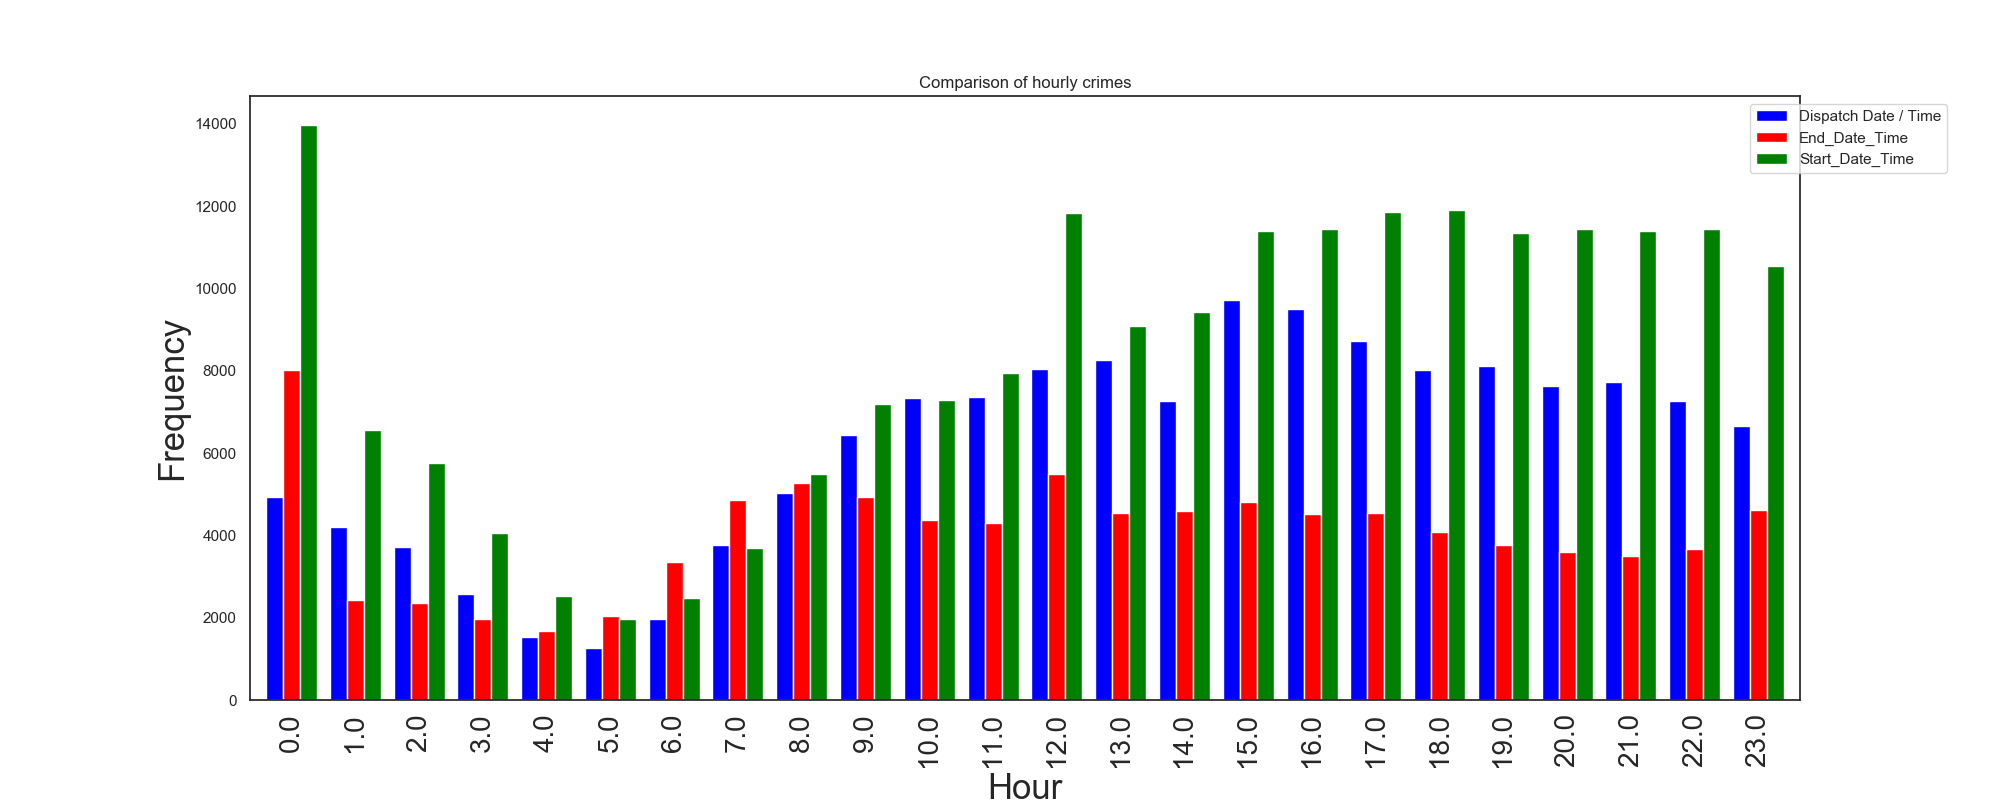
\includegraphics[width= 4.0 in]{crime_hour}
%\caption{$\Delta=0$}
\label{crimehour}
\end{figure}
Midnight outlier  for  \textcolor{red}{End}, and  \textcolor{OliveGreen}{Start} time data ?\\
Morning seems to have lesser crimes

\end{frame}
%------------------------------------------------
%------------------------------------------------
\begin{frame}
\frametitle{Crime month}
\begin{itemize}
%\item Which month/s? 
\item Again we use data from columns \textcolor{blue}{Dispatch},  \textcolor{red}{End}, and  \textcolor{OliveGreen}{Start} time data 
\end{itemize}
\graphicspath{{Figures//}}
\vspace{-0.5cm}
\begin{figure}[htbp]
%\begin{minipage}[b]{0.5\linewidth}
\centering
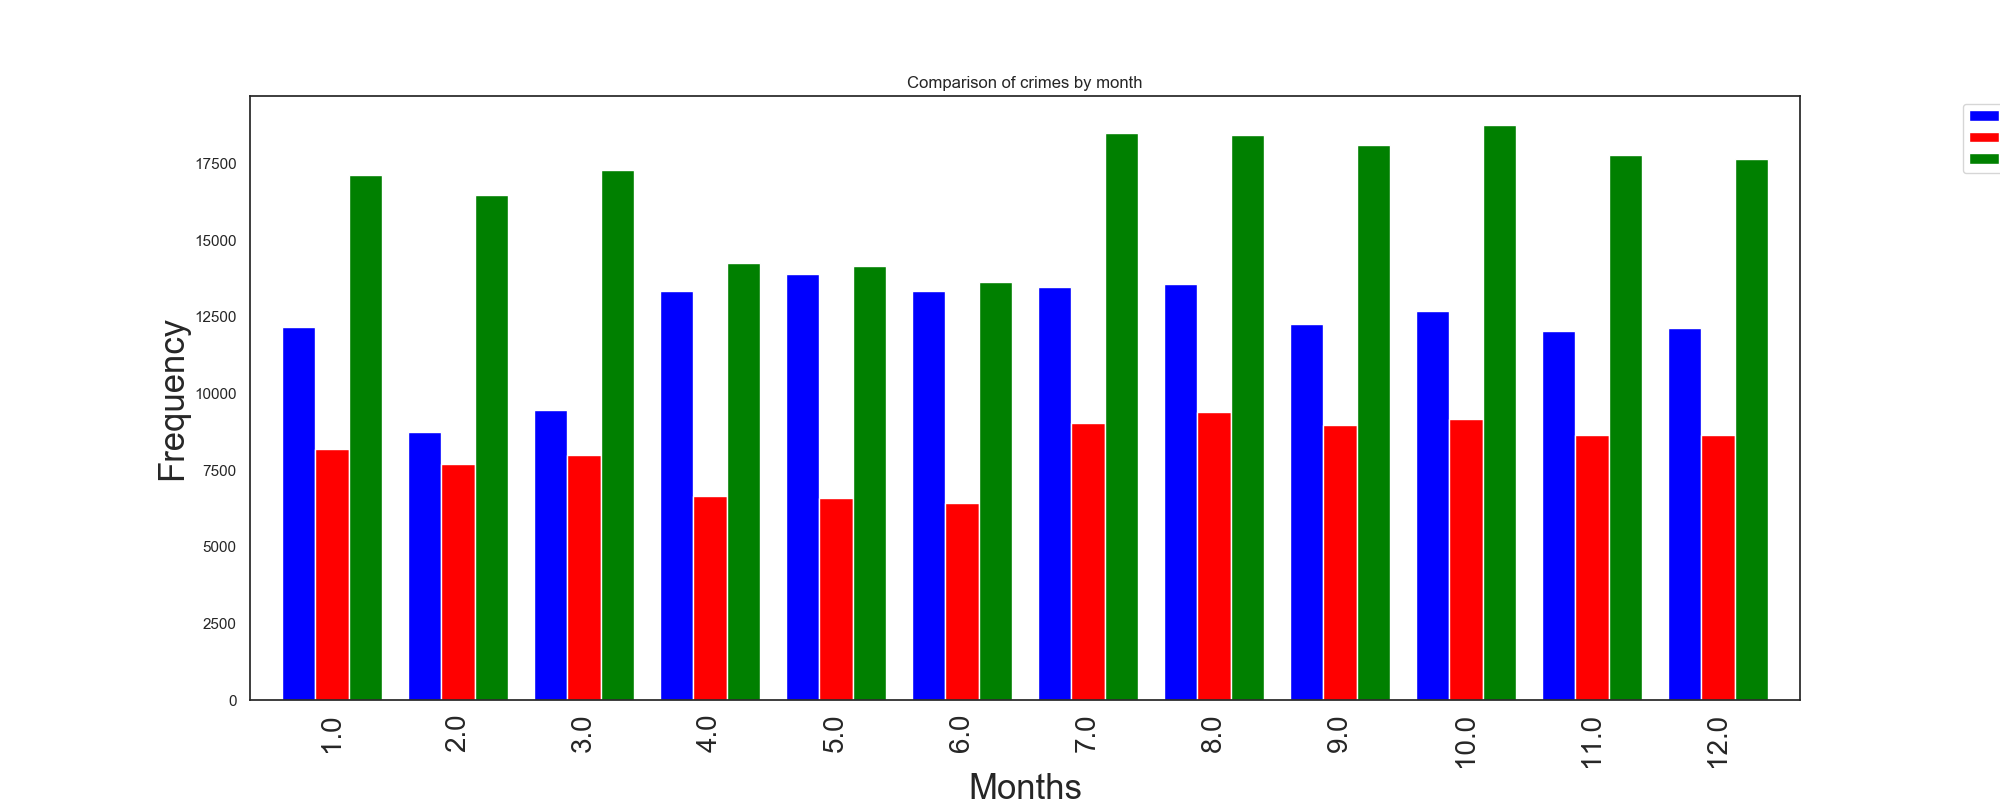
\includegraphics[width= 4.0 in]{crime_month}
%\caption{$\Delta=0$}
\label{crimemonthr}
\end{figure}
\textbf{April-June} for \textcolor{OliveGreen}{Start} \& \textcolor{red}{End} time approach, 
\textbf{February-March} for \textcolor{blue}{Dispatch} time approach, 
\end{frame}
%------------------------------------------------
%------------------------------------------------
\section{Locating Crime}
\subsection{The where of crime?}
%------------------------------------------------
\begin{frame}
\frametitle{Crimes by district}
%------------------------------------------------
\begin{block}{What we have}
We can use information about location, i.e Police District Name, Block Address, Zip Code, Sector, Beat, Latitude, Longitude, Police District Number, Location, Address Number
\end{block}
\begin{block}{for our purpose}
We chose to use Police District Name column as it has full information (i.e no missing values)
\end{block}
\begin{block}{ crime map?}
For future purpose one can use the other information to create a map displaying rates of crimes
\end{block}
\end{frame}
%------------------------------------------------
%------------------------------------------------
%\section{Results}
%------------------------------------------------
\begin{frame}
\frametitle{Crime by district}
%------------------------------------------------
\graphicspath{{Figures//}}
\vspace{-0.5cm}
\begin{figure}[htbp]
%\begin{minipage}[b]{0.5\linewidth}
\centering
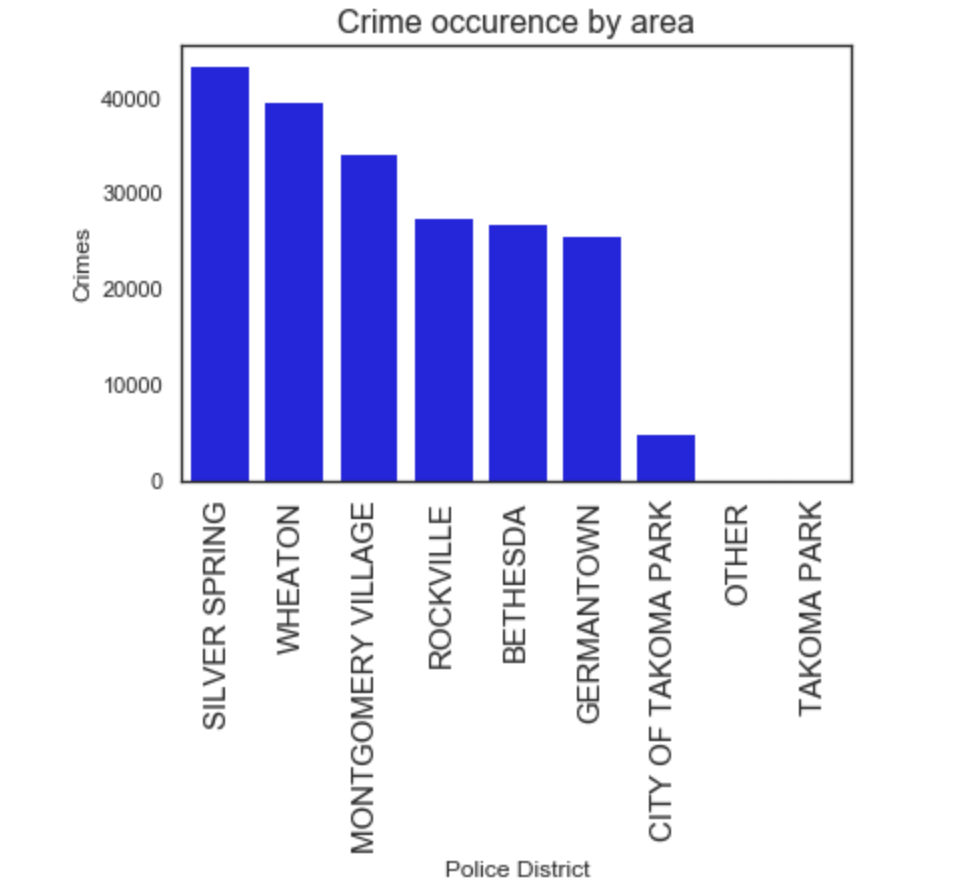
\includegraphics[width= 3.0 in]{crime_bydistrict}
%\caption{$\Delta=0$}
\label{crime_bydistrict.}
\end{figure}
\end{frame}
%------------------------------------------------
%------------------------------------------------
\begin{frame}
\frametitle{Crime by area}
%------------------------------------------------
\graphicspath{{Figures//}}
\vspace{-0.5cm}
\begin{figure}[htbp]
%\begin{minipage}[b]{0.5\linewidth}
\centering
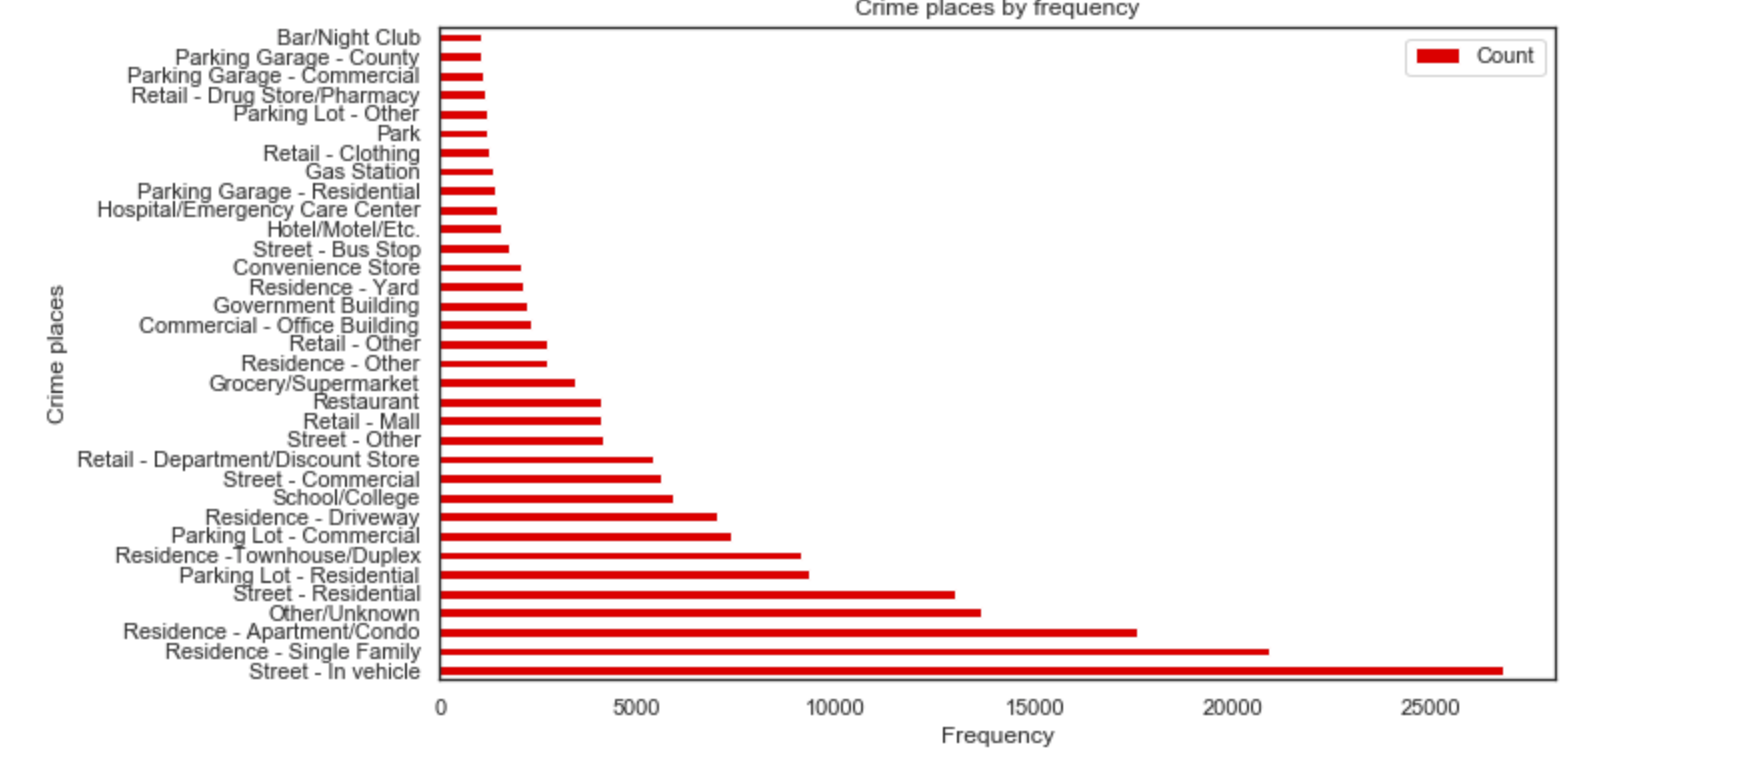
\includegraphics[width= 4.0 in]{crime_types}
%\caption{$\Delta=0$}
\label{crimetype}
\end{figure}
Low crime: Bar/Night Club, residential areas \textbf{high} crime place
\end{frame}
%------------------------------------------------
%------------------------------------------------
%------------------------------------------------
%------------------------------------------------
\section{Crime Types}
\subsection{Top five crimes}
%------------------------------------------------
\begin{frame}
\frametitle{Common crime types}
%------------------------------------------------
\begin{block}{How to get it}
We pivoted our data frame with index = Crime Name3, values = Incident ID  , then sort them by count 
\end{block}
\begin{tabular}{ |l|l| }
  \hline
  \multicolumn{2}{|c|}{Top five crime types} \\
  \hline
  Crime Name & Frequency \\
  \hline
  Larceny-from auto & 16811 \\
  Drugs-Marijuana-possess & 13983 \\
  Police Information & 11194 \\
  Driving under the influence of liquor & 10878 \\
  Assault- 2nd degree & 10858 \\
  \hline
  \end{tabular}
\end{frame}
%------------------------------------------------
%------------------------------------------------
\subsection{Bottom five crime types}
%------------------------------------------------
\begin{frame}
\frametitle{lowest crimes}
%------------------------------------------------

\begin{tabular}{ |l|l| }
  \hline
  \multicolumn{2}{|c|}{Bottom five crime types} \\
  \hline
  Crime Name & Frequency \\
  \hline
  Homicide- negligent manslaughter & 1 \\
  Compounding crime & 1 \\
  Condit release violation & 1 \\
  Conservation- animals (describe offense) & 1 \\
  Damage property- business-with explosive & 1 \\
  \hline
  \end{tabular}

\end{frame}
%------------------------------------------------
%------------------------------------------------
%------------------------------------------------
\begin{frame}
\frametitle{Conclusions}
%------------------------------------------------

\begin{itemize}
\item The beginning of the week was  the period most crimes (Monday, Tuesday and Wednesday). 
\item It is also seen  that February and March, have lesser crime incidents.
\item Most of the crimes committed are in and around Silver Spring district.
\item We also observed that the most crimes occur around residential places, and least crimes are committed in places like Bar/Club.
\item The most common crime is Larceny followed by drugs/marijuana possession.
\item The least crimes are crimes such as: homicide, damage property, etc.
\end{itemize}
\end{frame}
%-----------------------------------------------------------
%----------------------------------------------------------
\section{Conclusion}
%------------------------------------------------------
%----------------------------------------------------
%----------------------------------------------------
\begin{frame}
\frametitle{Limitation of the study}
%------------------------------------------------------

\begin{itemize}
\item Is it possible to determine the longest and shortest police response time? Does the response time vary from district to district?
\item It will be insightful and helpful to classify the types of crimes by whether they are violent or not.
\item Furthermore, a relevant information could be to know in which places there are more occurrences of crimes and in which shift these crimes are most common.
\item Further investigation is required to answer why 2016 registered low crimes.
\item Will we arrive at different conclusion if we make analysis based on  population density instead of district?
\end{itemize}
\end{frame}
%------------------------------------------------------
%------------------------------------------------
%------------------------------------------------
\begin{frame}
\Huge{\centerline{\textcolor{red}{Thank you for your attention}}}
\end{frame}
%------------------------------------------------
%------------------------------------------------


%----------------------------------------------------------------------------------------
\bibliographystyle{plain}
\bibliography{References}
\end{document} 